\documentclass[10pt,a4paper]{beamer}
				
\usepackage[ngerman]{babel}
\usepackage[T1]{fontenc}
\usepackage[utf8]{inputenc}
\usepackage{varioref}
\usepackage{hyperref}
\usepackage{cleveref}
\usepackage{amsmath}
\usepackage{amsfonts}
\usepackage{amssymb}
\usepackage{makeidx}
\usepackage{graphicx}
\usepackage{csquotes}
\usepackage{listings}
\usepackage{color}
\usepackage{xcolor}
\usepackage[most]{tcolorbox}
\usepackage{amssymb}
\usepackage{lmodern}
\usepackage{verbatim}

% Umlaute und ß in Listings
\lstset{basicstyle=\ttfamily}
\lstset{literate=%
  {Ö}{{\"O}}1
  {Ä}{{\"A}}1
  {Ü}{{\"U}}1
  {ß}{{\ss}}1
  {ü}{{\"u}}1
  {ä}{{\"a}}1
  {ö}{{\"o}}1
}

% Farben für Listings
\definecolor{codegreen}{rgb}{0,0.6,0}
\definecolor{codegray}{rgb}{0.5,0.5,0.5}
\definecolor{codepurple}{rgb}{0.58,0,0.82}
\definecolor{backcolour}{rgb}{0.95,0.95,0.92}
 
\lstdefinestyle{mystyle}{
    backgroundcolor=\color{backcolour},   
    commentstyle=\color{codegreen},
    keywordstyle=\color{magenta},
    numberstyle=\tiny\color{codegray},
    stringstyle=\color{codepurple},
    basicstyle=\footnotesize,
    breakatwhitespace=false,         
    breaklines=true,                 
    captionpos=t,                    
    keepspaces=true,                 
    numbers=left,                    
    numbersep=5pt,                  
    showspaces=false,                
    showstringspaces=false,
    showtabs=false,                  
    tabsize=2,
	language=sql
}
 
\lstset{style=mystyle}


\setbeamercolor{logo}{bg=white}  %controls the color of the logo area
\setbeamertemplate{navigation symbols}{}

\usetheme{PaloAlto}
\renewcommand{\footnotesize}{\small}
\newcommand{\pftn}[1]{\let\thefootnote\relax\footnotetext{\tiny #1}}
\newcommand{\ftn}[2]{\footnote[#1]{\tiny #2}}
\newenvironment{hlbox}{\begin{tcolorbox}[enhanced,colback=white,colframe=white,sharpish corners,fuzzy halo=0.5mm with lightgray]}{\end{tcolorbox}}

\logo{
\includegraphics[width=0.155\linewidth]{hbbk-logo}}
\author{Luca Kiebel}
\title{Mengenoperationen}
\subtitle{Zwei Abfragen zu einer zusammenfassen}
\date{\today}
\setlength{\itemsep}{10pt}
\begin{document}
\begin{frame}
\titlepage
\end{frame}

\begin{frame}
\frametitle{Inhaltsverzeichnis}\tableofcontents
\end{frame}

\section{Mengenoperationen}
\begin{frame}
\frametitle{Mengenoperationen}
\begin{itemize}
\item Dienen zur Zusammenfassung von Abfragen
\pause
\item Vereinigungsmenge: \lstinline|UNION|
\pause
\item Schnittmenge: \lstinline|INTERSECT|
\pause
\item Differenzmenge: \lstinline|MINUS|
\end{itemize}
\end{frame}

\section{Union}
\begin{frame}
\frametitle{Union}
Zur Vereinigung zweier Abfragemengen wird \lstinline|UNION| verwendet.
\newline
\begin{center}
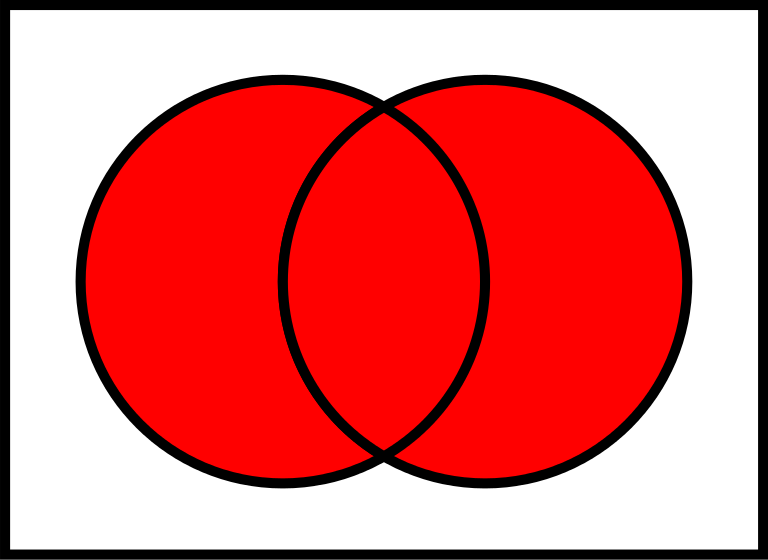
\includegraphics[width=0.5\linewidth]{vereinigungsmenge}
\end{center}
\end{frame}

\subsection{Syntax}
\begin{frame}[fragile]
\frametitle{Syntax}
\framesubtitle{Union}
\begin{lstlisting}
SELECT ausdruck1, ausdruck2, ... ausdruckN
FROM tabelle
UNION
SELECT ausdruck1, ausdruck2, ... ausdruckN
FROM tabelle
[ORDER BY ..]
\end{lstlisting}
\pause
\textbf{Wichtiges:}
\begin{itemize}
\item Beide Abfragen müssen gleich viele Ausdrücke enthalten
\item Die Spalten müssen den selben Datentypen haben 
\end{itemize}
\end{frame}

\subsection{Beispiel}
\begin{frame}[fragile]
\frametitle{Beispiel}
\framesubtitle{Union}
\begin{tabular}{l|l}
\textbf{verkaeufer\_id} & \textbf{verkaeufer\_name} \\ \hline
1000           & Samsung          \\
2000           & Apple            \\
3000           & Google           \\
4000           & Lenovo           \\
\end{tabular} 
\newline
\vspace*{1 cm}
\newline
\begin{tabular}{l|l|l}
\textbf{bestellung\_id} & \textbf{bestellung\_datum} & \textbf{verkaeufer\_id} \\ \hline
1              & 2018-01-01        & 2000           \\
2              & 2018-01-01        & 7000           \\
3              & 2018-01-02        & 8000           \\
\end{tabular}
\end{frame}

\begin{frame}[fragile]
\frametitle{Beispiel}
\framesubtitle{Union}
\begin{lstlisting}
SELECT verkaeufer_id 
FROM verkauefer
UNION
SELECT verkaeufer_id 
FROM bestellung
ORDER BY verkaeufer_id 
\end{lstlisting}
\pause
\begin{tabular}{l}
\textbf{verkaeufer\_id} \\ \hline
1000 \\
2000 \\
3000 \\
4000 \\
7000 \\ 
8000
\end{tabular}
\end{frame}

\subsection{Union All}
\begin{frame}[fragile]
\frametitle{Union All}
\framesubtitle{Union}
\lstinline|Union All| gibt mehrfach vorkommende Zeilen aus.  \\
\begin{lstlisting}
SELECT verkaeufer_id 
FROM verkauefer
UNION ALL
SELECT verkaeufer_id 
FROM bestellung
ORDER BY verkaeufer_id 
\end{lstlisting}
\pause
\begin{tabular}{l}
\textbf{verkaeufer\_id} \\ \hline
1000 \\
2000 \\
2000 \\
3000 \\
4000 \\
7000 \\ 
8000
\end{tabular}
\end{frame}

\begin{frame}[fragile]
\frametitle{Beispiel}
\framesubtitle{Union All}
\begin{tabular}{l|l}
\textbf{verkaeufer\_id} & \textbf{verkaeufer\_name} \\ \hline
1000           & Samsung          \\
2000           & Apple            \\
3000           & Google           \\
4000           & Lenovo           \\
\end{tabular} 
\newline
\vspace*{1 cm}
\newline
\begin{tabular}{l|l|l}
\textbf{bestellung\_id} & \textbf{bestellung\_datum} & \textbf{verkaeufer\_id} \\ \hline
1              & 2018-01-01        & 2000           \\
2              & 2018-01-01        & 7000           \\
3              & 2018-01-02        & 8000           \\
\end{tabular}
\end{frame}

\section{Intersect}
\begin{frame}
\frametitle{Intersect}
Zum Ausgeben der Schnittmenge zweier Abfragen wird \lstinline|INTERSECT| verwendet.
\begin{center}
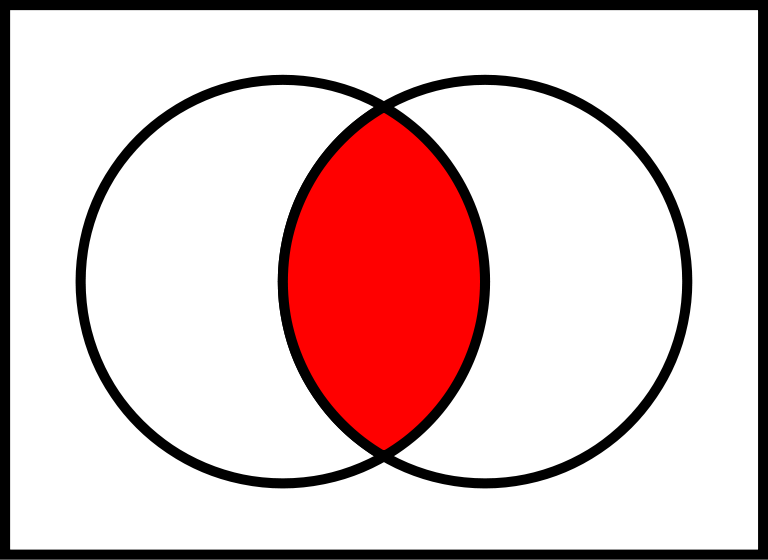
\includegraphics[width=0.5\linewidth]{schnittmenge}
\end{center}
\end{frame}

\subsection{Syntax}
\begin{frame}[fragile]
\frametitle{Syntax}
\framesubtitle{Intersect}
\begin{lstlisting}
SELECT ausdruck1, ausdruck2, ... ausdruckN
FROM tabelle
INTERSECT	
SELECT ausdruck1, ausdruck2, ... ausdruckN
FROM tabelle
[ORDER BY ..]
\end{lstlisting}
\textbf{Wichtiges:}
\begin{itemize}
\item Beide Abfragen müssen gleich viele Ausdrücke enthalten
\item Die Spalten müssen den selben Datentypen haben 
\end{itemize}
\end{frame}

\subsection{Beispiel}
\begin{frame}[fragile]
\frametitle{Beispiel}
\framesubtitle{Intersect}
\begin{tabular}{l|l}
\textbf{verkaeufer\_id} & \textbf{verkaeufer\_name} \\ \hline
1000           & Samsung          \\
2000           & Apple            \\
3000           & Google           \\
4000           & Lenovo           \\
\end{tabular} 
\newline
\vspace*{1 cm}
\newline
\begin{tabular}{l|l|l}
\textbf{bestellung\_id} & \textbf{bestellung\_datum} & \textbf{verkaeufer\_id} \\ \hline
1              & 2018-01-01        & 2000           \\
2              & 2018-01-01        & 7000           \\
3              & 2018-01-02        & 8000           \\
\end{tabular}
\end{frame}

\begin{frame}[fragile]
\frametitle{Beispiel}
\framesubtitle{Intersect}
Alle bekannten Verkäufer mit verkauften Produkten: \\
\begin{lstlisting}
SELECT verkaeufer_id
FROM veraeufer
INTERSECT
SELECT verkaeufer_id
FROM bestellung
ORDER BY verkaeufer_id
\end{lstlisting}
\pause
\begin{tabular}{l}
\textbf{verkaeufer\_id} \\ \hline
2000
\end{tabular}
\end{frame}

\subsection{Beispiel (MySQL)}
\begin{frame}[fragile]
\frametitle{Beispiel (MySQL)}
\framesubtitle{Intersect}
Da \lstinline|INTERSECT| nicht in MySQL enthalten ist, müssen hier Workarounds gefunden werden:
\pause
\begin{lstlisting}
SELECT verkaeufer_id 
FROM verkaeufer
INNER JOIN bestellung
ON verkaeufer.verkaeufer_id = bestellung.verkaeufer_id
\end{lstlisting}
\pftn{https://blog.codinghorror.com/a-visual-explanation-of-sql-joins/}
\pause
\begin{tabular}{l}
\textbf{verkaeufer\_id} \\ \hline
2000
\end{tabular}

\end{frame}

\section{Minus}
\begin{frame}
\frametitle{Minus}
Zum Ausgeben aller Datensätze, die ausschließlich in einer von zwei Tabellen sind, wird \lstinline|MINUS| genutzt. 
\begin{center}
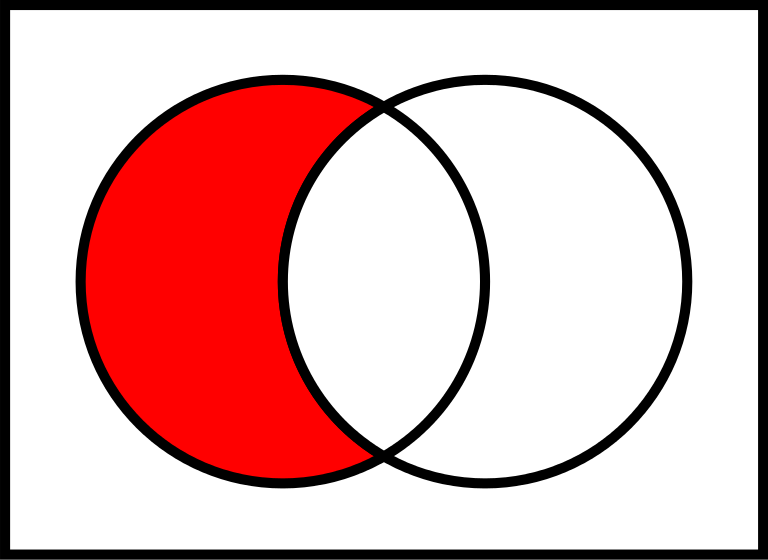
\includegraphics[width=0.5\linewidth]{differenzmenge}
\end{center}
\end{frame}

\subsection{Syntax}
\begin{frame}[fragile]
\frametitle{Syntax}
\framesubtitle{Minus}
\begin{lstlisting}
SELECT ausdruck1, ausdruck2, ... ausdruckN
FROM tabelle
MINUS
SELECT ausdruck1, ausdruck2, ... ausdruckN
FROM tabelle
[ORDER BY ..]
\end{lstlisting}
\textbf{Wichtiges:}
\begin{itemize}
\item Beide Abfragen müssen gleich viele Ausdrücke enthalten
\item Die Spalten müssen den selben Datentypen haben 
\end{itemize}
\end{frame}

\subsection{Beispiel}
\begin{frame}[fragile]
\frametitle{Beispiel}
\framesubtitle{Minus}
\begin{tabular}{l|l}
\textbf{verkaeufer\_id} & \textbf{verkaeufer\_name} \\ \hline
1000           & Samsung          \\
2000           & Apple            \\
3000           & Google           \\
4000           & Lenovo           \\
\end{tabular} 
\newline
\vspace*{1 cm}
\newline
\begin{tabular}{l|l|l}
\textbf{bestellung\_id} & \textbf{bestellung\_datum} & \textbf{verkaeufer\_id} \\ \hline
1              & 2018-01-01        & 2000           \\
2              & 2018-01-01        & 7000           \\
3              & 2018-01-02        & 8000           \\
\end{tabular}
\end{frame}

\begin{frame}[fragile]
\frametitle{Beispiel}
\framesubtitle{Minus}
Alle bekannten Verkäufer, die noch kein Produkt verkauft haben: \\
\begin{lstlisting}
SELECT verkaeufer_id
FROM verkaeufer
MINUS
SELECT verkaeufer_id
FROM bestellung
ORDER BY verkaeufer_id
\end{lstlisting}
\pause
\begin{tabular}{l}
\textbf{verkaeufer\_id} \\ \hline
1000 \\
3000 \\
4000 \\
\end{tabular}
\end{frame}

\subsection{Beispiel (MySQL)}
\begin{frame}[fragile]
\frametitle{Beispiel (MySQL)}
\framesubtitle{Minus}
\lstinline|MINUS| ist ebenfalls nicht in MySQL enthalten. Hier lässt sich zum Glück auch einfach eine Lösung finden: \pause
\begin{lstlisting}
SELECT verkaeufer_id 
FROM verkaeufer
LEFT OUTER JOIN bestellung
ON verkaeufer.verkaeufer_id = bestellung.verkaeufer_id
WHERE bestellung.verkaeufer_id IS NULL
\end{lstlisting}
\pftn{https://blog.codinghorror.com/a-visual-explanation-of-sql-joins/}
\pause
\begin{tabular}{l}
\textbf{verkaeufer\_id} \\ \hline
1000 \\
3000 \\
4000 \\
\end{tabular}
\end{frame}

\section{ }
\begin{frame}
\titlepage
\end{frame}

\end{document}